\section{Floor Grid}\label{sec:floor-grid}

As suggested in the studies examined in section~\ref{subsec:stable-reference-frame}, we decided to add a stable
reference frame to help with postural stability.
Especially, we focus on the 6-Degrees-of-Freedom navigation in the interplanetary areas of the Simulation, that
generally lack any sort of fixed reference frame, since movement on a planet surface has the surface and its normal
direction as a strong visual indicator for a reference frame.
The Floor grid aims to provide a definitive up-direction that is parallel to the real world's gravity, thereby
improving postural stability and minimizing sensory conflicts.
While superimposing a grid on the floor may significantly reduce the feeling of presence, we accept this effect since
the primary function of CosmoScout VR as a scientific visualization tool is not as dependent on an immersive feeling
as entertainment oriented simulations may be.
Additionally, we also suspect that small changes to the control scheme can be done to further change the interaction
context from an egocentric view within the simulation to a more exocentric "Pseudo AR" approach, where the user
manipulates the surrounding simulation without moving, similar to the Worlds-in-Miniature approach proposed
by Drogemuller et al.~\cite{Drogemuller2020}.
The Hypothesis is that a "Pseudo AR" simulation environment would drastically reduce cybersickness symptoms, as the
sensory conflict between the user inside the simulation and the real world is minimal, and maintaining postural
stability should be easier for the user.
Additionally, the best practices mentioned by McCauley et al.~\cite{McCauley1992}, include that users should be
considered
individually as reaction and adaptation to virtual environments are different for each case.
In order to match individual users adaptation progress, as well as different scenarios regarding the hardware setup,
most values and aspects of the grid can be customised through the settings file and almost all of them are also
changeable in the options menu at runtime.

\subsection{Floor Grid Implementation}\label{subsec:floor-grid-implementation}

\begin{figure}[h]
    \centering
    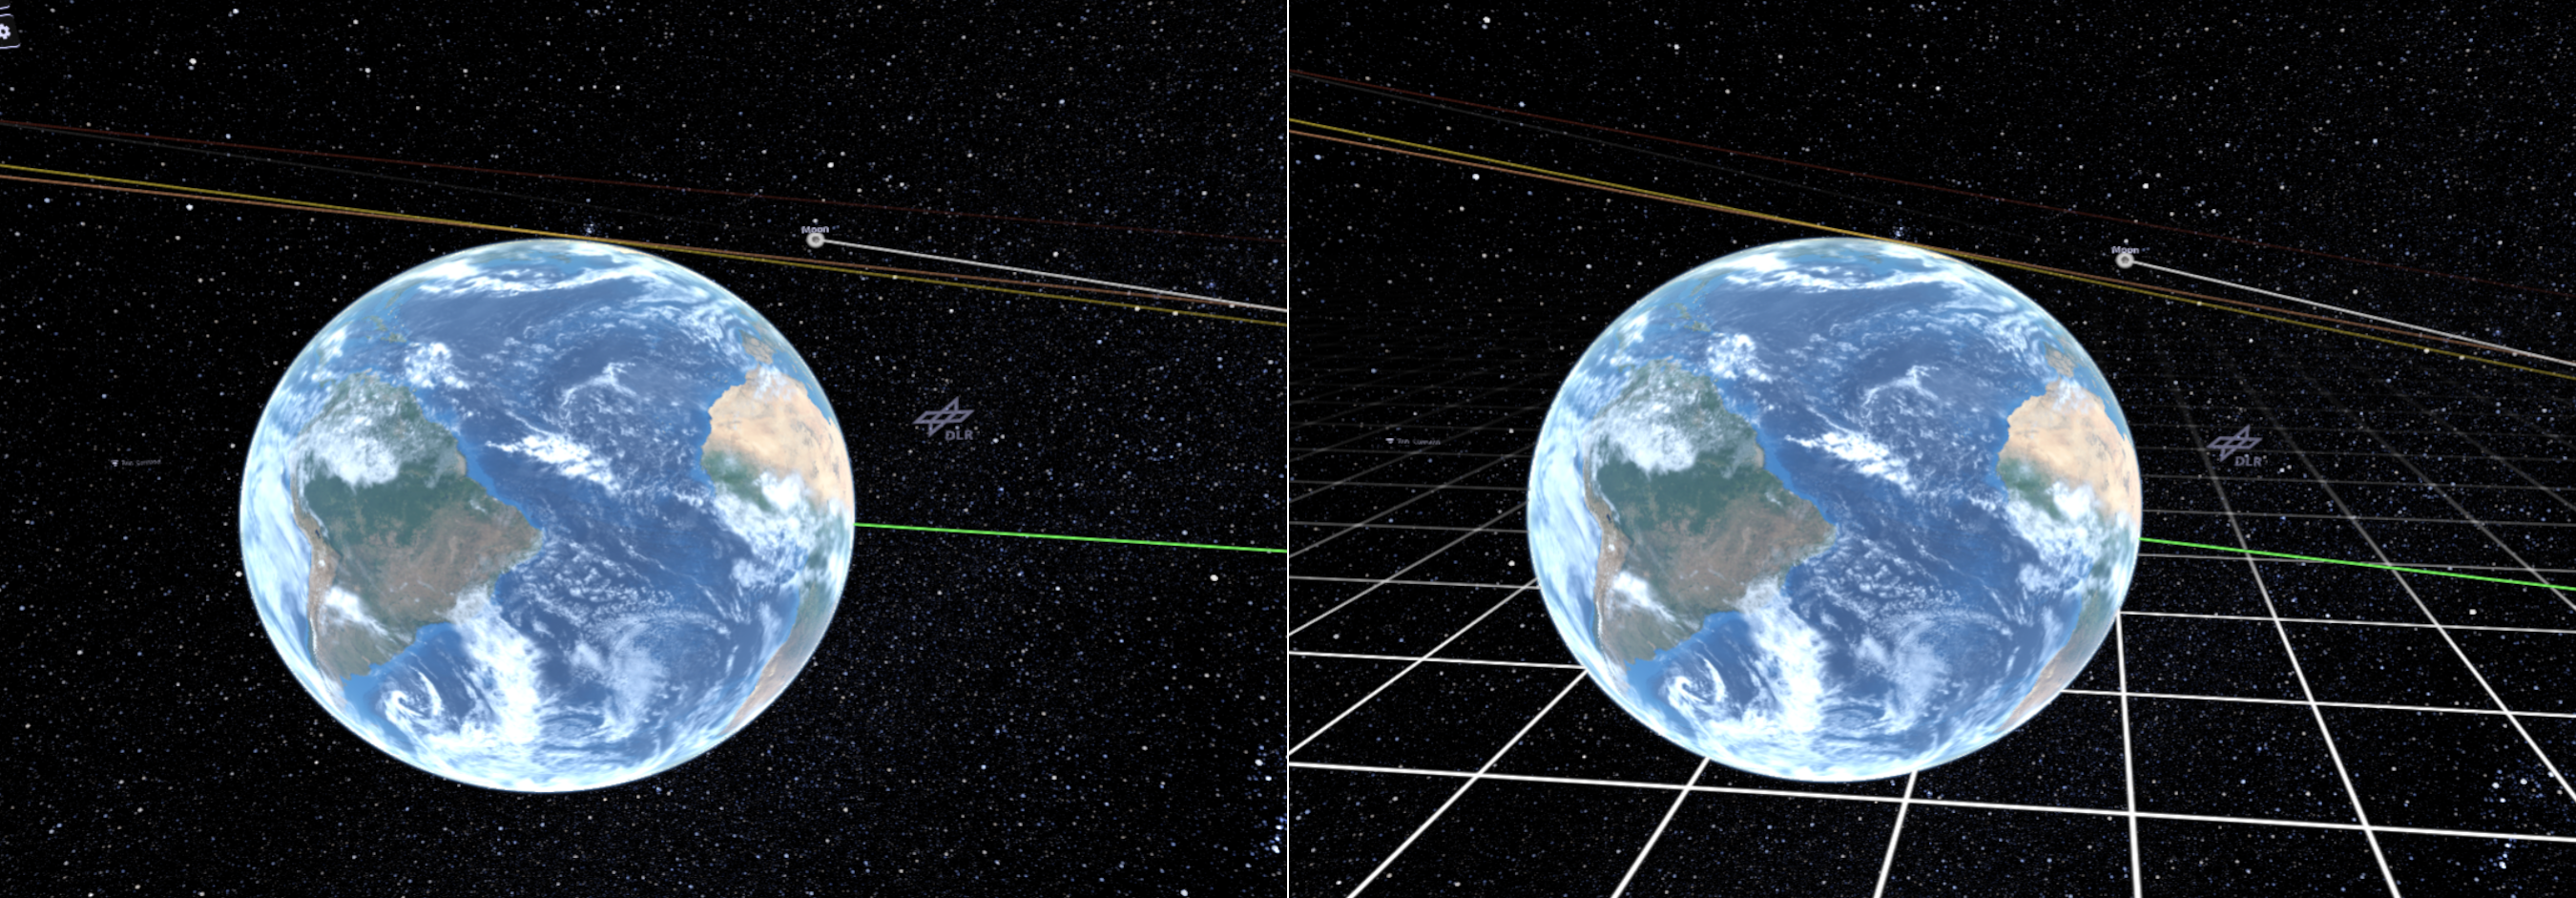
\includegraphics[width=\textwidth]{content/4_1_floorGrid/img/FloorGrid_Screenshot}
    \caption{Screenshot of CosmoScout VR with (right) and without (left) the Floor Grid.}
    \label{fig:floor-grid-screenshot}
\end{figure}
The Floor Grid is implemented in the VR Accessibility Plugin for CosmoScout VR.
This way it can be optionally loaded with CosmoScout when it is needed.
It renders a quad that is fixed to the observer's position and GUI elements.
This way still allows free movements with the VR HMD while staying a static frame of reference that is tied to
the real world floor.
To properly adjust the grid to the real world floor the node drawing the quad is attached to the node drawing the GUI
via a transform node in the scenegraph that adds a vertical offset (in meters) to the grid that is adjustable in the
settings file before startup, and the options menu at runtime.
The quad size is defined in the settings file as a multiplier (\textit{uFalloff} / \textit{gridFalloff}) that scales
the initial quad, spanning in x and y direction from -1 to 1, up by the value set in the settings file.
The scaled quad is textured with a semi transparent texture containing the grid with the center of the grid either as a
square or a cross.
Additionally, the texture can be scaled by a separate factor (\textit{uSize} / \textit{gridSize}) resulting in a
coarser or finer mesh.
The calculations for the vertex positions and texture coordinates are shown in the code block below from the Floor
Grid's vertex shader:
\begin{minted}{c}
    void main()
    {
        vTexCoords  = vec2( (iQuadPos.x + 1)/2 * uFalloff * uSize,
                            (iQuadPos.y + 1)/2 * uFalloff * uSize );

        vPosition   = (uMatModelView * vec4(iQuadPos.x * uFalloff, 0.0, iQuadPos.y * uFalloff, 1.0)).xyz;
        gl_Position = uMatProjection * vec4(vPosition, 1);
    }
\end{minted}
The variables \textit{uMatModelView} and \textit{uMatProjection} are the Model, View, and Projection Matrices needed
to transform the coordinates in the graphics pipeline.
The Floor Grid's fragment shader applies the selected texture, but is discarded if the fragment is not part of a grid
line (i.e.\ is fully transparent).
Additionally, the texture's opacity (\textit{uAlpha} / \textit{gridAlpha}) is adjustable through the settings file and
in the options menu at runtime.
To prevent aliasing or the grid turning into a grey plane towards the horizon, the floor grid is drawn with the
OpenGL Blend Function "\mintinline{c}{glBlendFunc(GL_SCR_ALPHA, GL_ONE_MINUS_SRC_ALPHA)}".
This blend function leads to the grid fading after a few meters because the texture is mostly transparent.
finally the color of the grid is adjustable in the settings file or in the options at runtime to allow more
customisation for individual users.
Figure~\ref{fig:floor-grid-screenshot} shows a screenshot of the floor grid in use compared to the same scene without
the grid.
